\documentclass[12pt, titlepage]{article}

\usepackage{fullpage}
\usepackage[round]{natbib}
\usepackage{multirow}
\usepackage{booktabs}
\usepackage{tabularx}
\usepackage{graphicx}
\usepackage{float}
\usepackage{hyperref}
\hypersetup{
    colorlinks,
    citecolor=blue,
    filecolor=black,
    linkcolor=red,
    urlcolor=blue
}

\usepackage{tikz}
\usetikzlibrary{positioning}

\input{../../Comments}
%% Common Parts

\newcommand{\progname}{The Crazy Tens} % PUT YOUR PROGRAM NAME HERE
\newcommand{\authname}{Team \#25, The Crazy Four
\\Ruida Chen
\\Ammar Sharbat 
\\Alvin Qian
\\Jiaming Li} % AUTHOR NAMES                  

\usepackage{hyperref}
    \hypersetup{colorlinks=true, linkcolor=blue, citecolor=blue, filecolor=blue,
                urlcolor=blue, unicode=false}
    \urlstyle{same}
                                


\newcounter{acnum}
\newcommand{\actheacnum}{AC\theacnum}
\newcommand{\acref}[1]{AC\ref{#1}}

\newcounter{ucnum}
\newcommand{\uctheucnum}{UC\theucnum}
\newcommand{\uref}[1]{UC\ref{#1}}

\newcounter{mnum}
\newcommand{\mthemnum}{M\themnum}
\newcommand{\mref}[1]{M\ref{#1}}

\begin{document}

\title{Module Guide for The Crazy Four} 
\author{
    Team \#25, The Crazy Four \\[1ex]
    Ruida Chen \\
    Ammar Sharbat \\
    Alvin Qian \\
    Jiaming Li
}
\date{\today}

\maketitle

\pagenumbering{roman}

\section{Revision History}

\begin{tabularx}{\textwidth}{p{3cm}p{2cm}X}
\toprule {\bf Date} & {\bf Version} & {\bf Notes}\\
\midrule
Nov 6 & Alvin, Ammar, Ruida, Jim & Initial draft of basic MG (not in report)\\
Nov 7 & Above \& Chris Schankula & Review and feedback of basic MG\\
Nov 8 & Alvin & Module Hierarchy and decomposition\\
Nov 9 & Alvin & Updated API's for game action modules\\
Nov 13 & Alvin & modified module decomposition to remove incorrect content\\
Nov 13 & Ammar & added ACs, AC Traceability, Use Hierarchy, UI, Design of CPs; WebSocket, Timeline\\
\bottomrule
\end{tabularx}

\newpage

\section{Reference Material}

This section records information for easy reference.

\subsection{Abbreviations and Acronyms}

\renewcommand{\arraystretch}{1.2}
\begin{tabular}{l l} 
  \toprule     
  \textbf{symbol} & \textbf{description}\\
  \midrule 
  AC & Anticipated Change\\
  ACID & Atomicity, Consistency, Isolation, Durability\\
  API & Application Programming Interface\\
  CSS & Cascading Style Sheets\\
  DAG & Directed Acyclic Graph \\
  DOM & Document Object Model\\
  FR & Functional Requirement\\
  HTTP & Hypertext Transfer Protocol\\
  JSON & JavaScript Object Notation\\
  JWT & JSON Web Token\\
  M & Module \\
  MG & Module Guide \\
  NFR & Non-Functional Requirement\\
  OS & Operating System \\
  R & Requirement\\
  REST & Representational State Transfer\\
  SC & Scientific Computing \\
  SR & Safety Requirement\\
  SRS & Software Requirements Specification\\
  SQL & Structured Query Language\\
  UC & Unlikely Change \\
  UI & User Interface\\
  \bottomrule
\end{tabular}\\

\newpage

\tableofcontents

\listoftables

\listoffigures

\newpage

\pagenumbering{arabic}

\section{Introduction}

Decomposing a system into modules is a commonly accepted approach to developing
software.  A module is a work assignment for a programmer or programming
team~\citep{ParnasEtAl1984}.  We advocate a decomposition
based on the principle of information hiding~\citep{Parnas1972a}.  This
principle supports design for change, because the ``secrets'' that each module
hides represent likely future changes.  Design for change is valuable in SC,
where modifications are frequent, especially during initial development as the
solution space is explored.  

Our design follows the rules layed out by \citet{ParnasEtAl1984}, as follows:
\begin{itemize}
\item System details that are likely to change independently should be the
  secrets of separate modules.
\item Each data structure is implemented in only one module.
\item Any other program that requires information stored in a module's data
  structures must obtain it by calling access programs belonging to that module.
\end{itemize}

After completing the first stage of the design, the Software Requirements
Specification (SRS), the Module Guide (MG) is developed~\citep{ParnasEtAl1984}. The MG
specifies the modular structure of the system and is intended to allow both
designers and maintainers to easily identify the parts of the software.  The
potential readers of this document are as follows:

\begin{itemize}
\item New project members: This document can be a guide for a new project member
  to easily understand the overall structure and quickly find the
  relevant modules they are searching for.
\item Maintainers: The hierarchical structure of the module guide improves the
  maintainers' understanding when they need to make changes to the system. It is
  important for a maintainer to update the relevant sections of the document
  after changes have been made.
\item Designers: Once the module guide has been written, it can be used to
  check for consistency, feasibility, and flexibility. Designers can verify the
  system in various ways, such as consistency among modules, feasibility of the
  decomposition, and flexibility of the design.
\end{itemize}

The rest of the document is organized as follows. Section
\ref{SecChange} lists the anticipated and unlikely changes of the software
requirements. Section \ref{SecMH} summarizes the module decomposition that
was constructed according to the likely changes. Section \ref{SecConnection}
specifies the connections between the software requirements and the
modules. Section \ref{SecMD} gives a detailed description of the
modules. Section \ref{SecTM} includes two traceability matrices. One checks
the completeness of the design against the requirements provided in the SRS. The
other shows the relation between anticipated changes and the modules. Section
\ref{SecUse} describes the use relation between modules.


\section{Anticipated and Unlikely Changes (completed)} \label{SecChange}

This section lists the project changes that we expect (``Likely Changes'') and those we consider unlikely within the capstone timeframe (``Unlikely Changes'').  Where applicable each anticipated change (AC) has been given an identifier to support traceability and to guide module secrets.

\subsection{Likely Changes (each becomes an AC / module secret)}
\begin{description}
  \item[\refstepcounter{acnum}\label{acRules} \actheacnum\ --- Rule Engine Changes:] 
    The validation and behavioural details of the game's rule engine (e.g., how special cards behave, new house rules or alternate base arithmetic rules).  
    \\
    \textbf{Rationale:} Rules are likely to be refined during playtesting and instructor feedback, so they should be isolated in the \mref{mRules} module.

  \item[\refstepcounter{acnum}\label{acBases} \actheacnum\ --- Numeric Base Support (Dozenal and beyond):] 
    Support for additional numeral systems (Octal, Hex, etc.), and how scores and hints convert and present values.  
    \\
    \textbf{Rationale:} We intend the product to be extensible to multiple bases; the conversion logic and scoring changes must be encapsulated in \mref{mBaseConversion}, \mref{mScoring}, and \mref{mScoreboardView}.

  \item[\refstepcounter{acnum}\label{acScoring} \actheacnum\ --- Scoring Formula / Presentation:] 
    Changes to how round or match scoring is calculated, aggregated or displayed (e.g., bonus rules, alternate tallying).  
    \\
    \textbf{Rationale:} Scoring may evolve after playtests; keep scoring logic isolated in \mref{mScoring}.

  \item[\refstepcounter{acnum}\label{acUI} \actheacnum\ --- UI and Interaction Patterns:] 
    Layout, hint presentation, animations, accessibility adaptations, and onboarding flow.  
    \\
    \textbf{Rationale:} UI polish and accessibility tweaks are frequent after usability sessions; the \mref{mAppShell}, \mref{mGameBoardView}, and \mref{mMoveController} should hide these secrets.

  \item[\refstepcounter{acnum}\label{acSchema} \actheacnum\ --- Database Schema and Persistence Details:] 
    Changes to the persistent schema (profiles, history, telemetry format) and indexes.  
    \\
    \textbf{Rationale:} Data collection needs evolve; the \mref{mRepository} module hides these details.

  \item[\refstepcounter{acnum}\label{acRealtime} \actheacnum\ --- Real-time Messaging Strategy:] 
    Room lifecycle, message batching, reconnection rules, and state-resync semantics.  
    \\
    \textbf{Rationale:} Real-time policies affect multiplayer stability; isolate them in \mref{mRealtimeGateway} and \mref{mRealtimeClient}.

  \item[\refstepcounter{acnum}\label{acAuth} \actheacnum\ --- Authentication and Session Policies:] 
    Token lifetime, guest-session semantics, password storage scheme, and auth flows.  
    \\
    \textbf{Rationale:} Security/configuration choices can change; these are hidden by \mref{mAuth} and the \mref{mAPI} interface.
\end{description}

\subsection{Unlikely Changes (explicitly documented)}
These items are not expected to change during the capstone, so they are \emph{not} treated as module secrets and are documented rather than encapsulated in a separate module secret:

\begin{itemize}
  \item \textbf{Target Runtime Platforms:} Modern desktop browsers remain the deployment target for the deliverable.
  \item \textbf{Primary Tech Stack:} Web frontend framework, Server-side JavaScript runtime, Relational database for persistence.
  \item \textbf{Core Gameplay Pattern:} The turn-based matching mechanics (match by suit / match by value / sum-to-12 in Dozenal) are a stable product decision.
  \item \textbf{Non-functional goals baseline:} Performance targets (sub-300 ms updates), basic security expectations (TLS usage for network), and the expectation of GitHub-based CI.
\end{itemize}

\newpage

\section{Module Hierarchy} \label{SecMH}

This section provides an overview of the module design. Modules are summarized
in a hierarchy decomposed by secrets in Table \ref{TblMH}. The modules listed
below, which are leaves in the hierarchy tree, are the modules that will
actually be implemented.


\begin{description}
% --- Backend Modules ---
\item [\refstepcounter{mnum} \mthemnum \label{mAPI}:] API Module
    \begin{itemize}
        \item Provides stateless HTTP (REST) endpoints for auth and profile management. Active gameplay is handled separately via the Real-time Gateway.
    \end{itemize}

\item [\refstepcounter{mnum} \mthemnum \label{mRealtimeGateway}:] Real-time Gateway Module
    \begin{itemize}
        \item Manages stateful WebSocket connections for live gameplay and state syncing.
    \end{itemize}

\item [\refstepcounter{mnum} \mthemnum \label{mMatchmaking}:] Matchmaking Module
    \begin{itemize}
        \item Handles game lobby creation, joining, and starting a match.
    \end{itemize}

\item [\refstepcounter{mnum} \mthemnum \label{mAuth}:] Authentication Module
    \begin{itemize}
        \item Manages user identity, password hashing, and session token generation.
    \end{itemize}

\item [\refstepcounter{mnum} \mthemnum \label{mRepository}:] Repository Module
    \begin{itemize}
        \item Abstracts all database queries (SQL) and schema details for creating, reading, updating, and deleting data.
    \end{itemize}

\item [\refstepcounter{mnum} \mthemnum \label{mAudit}:] Audit Module
    \begin{itemize}
        \item Logs important server-side events for debugging and security.
    \end{itemize}

% --- Frontend Modules ---
\item [\refstepcounter{mnum} \mthemnum \label{mRealtimeClient}:] Real-time Client Module
    \begin{itemize}
        \item Establishes and maintains the client-side WebSocket connection; sends/receives game events.
    \end{itemize}

\item [\refstepcounter{mnum} \mthemnum \label{mAppShell}:] Application Shell Module
    \begin{itemize}
        \item The main component providing global layout, navigation, and state.
    \end{itemize}

\item [\refstepcounter{mnum} \mthemnum \label{mAuthClient}:] Authentication Client Module
    \begin{itemize}
        \item Provides the UI and logic for login/signup forms.
    \end{itemize}

\item [\refstepcounter{mnum} \mthemnum \label{mLobbyView}:] Lobby View Module
    \begin{itemize}
        \item UI component for displaying, creating, and joining game lobbies.
    \end{itemize}

\item [\refstepcounter{mnum} \mthemnum \label{mGameBoardView}:] Game Board View Module
    \begin{itemize}
        \item UI component that renders the main game interface (hands, deck, discard pile).
    \end{itemize}

\item [\refstepcounter{mnum} \mthemnum \label{mMoveController}:] Move Controller Module
    \begin{itemize}
        \item Manages user input (e.g., card clicks) and highlights valid moves.
    \end{itemize}

\item [\refstepcounter{mnum} \mthemnum \label{mScoreboardView}:] Scoreboard View Module
    \begin{itemize}
        \item UI component for displaying end-of-round scores in decimal and Dozenal.
    \end{itemize}

\item [\refstepcounter{mnum} \mthemnum \label{mProfileView}:] Profile View Module
    \begin{itemize}
        \item UI component for displaying user statistics and game history.
    \end{itemize}

% --- Core/Behaviour Modules ---
\item [\refstepcounter{mnum} \mthemnum \label{mGameEngine}:] Game Engine Module
    \begin{itemize}
        \item Manages the core game state (deck, hands) and turn progression.
    \end{itemize}

\item [\refstepcounter{mnum} \mthemnum \label{mRules}:] Rules Module
    \begin{itemize}
        \item Stateless logic to validate moves (e.g., match suit, rank, or Dozenal sum).
    \end{itemize}

\item [\refstepcounter{mnum} \mthemnum \label{mScoring}:] Scoring Module
    \begin{itemize}
        \item Calculates scores at the end of a round.
    \end{itemize}

\item [\refstepcounter{mnum} \mthemnum \label{mBaseConversion}:] Base Conversion Module
    \begin{itemize}
        \item Utility to convert numbers between decimal and Dozenal.
    \end{itemize}

\item [\refstepcounter{mnum} \mthemnum \label{mGameActions}:] Game Actions Module
    \begin{itemize}
        \item Defines types and structure for player actions (play card, draw, declare suit, submit score tally).
    \end{itemize}
\end{description}

\begin{table}[H]
\centering
\begin{tabular}{p{0.3\textwidth} p{0.3\textwidth} p{0.3\textwidth}}
\toprule
\textbf{Level 1} & \textbf{Level 2} & \textbf{Level 3 (Leaf Modules)}\\
\midrule

\multirow{1}{0.3\textwidth}{Hardware-Hiding Module} & ~ & (None) \\
\midrule

\multirow{5}{0.3\textwidth}{Behaviour-Hiding Module} & (Core Domain Logic) & \mref{mGameEngine} \\
& & \mref{mRules} \\
& & \mref{mScoring} \\
& & \mref{mBaseConversion} \\
& & \mref{mGameActions} \\
\midrule

\multirow{15}{0.3\textwidth}{Software Decision Module} & \multirow{6}{0.3\textwidth}{Backend (Server)} & \mref{mAPI} \\
& & \mref{mRealtimeGateway} \\
& & \mref{mMatchmaking} \\
& & \mref{mAuth} \\
& & \mref{mRepository} \\
& & \mref{mAudit} \\
\cmidrule{2-3}
& \multirow{9}{0.3\textwidth}{Frontend (Client)} & \mref{mRealtimeClient} \\
& & \mref{mAppShell} \\
& & \mref{mAuthClient} \\
& & \mref{mLobbyView} \\
& & \mref{mGameBoardView} \\
& & \mref{mMoveController} \\
& & \mref{mScoreboardView} \\
& & \mref{mProfileView} \\
\bottomrule

\end{tabular}
\caption{Module Hierarchy}
\label{TblMH}
\end{table}

\section{Connection Between Requirements and Design} \label{SecConnection}

The design of the system is intended to satisfy the requirements developed in
the SRS. In this stage, the system is decomposed into modules. The connection
between requirements and modules is listed in Table~\ref{TblRT}.\\


The design of the system is intended to satisfy the requirements developed in
the SRS. In this stage, the system is decomposed into modules. The connection
between requirements and modules is listed in the Traceability Matrix in Section \ref{SecTM} (Table \ref{TblRT}). This decomposition ensures that each Functional Requirement (FR), Non-functional Requirement (NFR), and Safety Requirement (SR) has a clear owner in the design, facilitating implementation and verification.

For example, core gameplay logic (FR-1 to FR-5) is satisfied by the \mref{mGameEngine} and \mref{mRules} modules, while the user-facing presentation (FR-7, FR-9) is handled by frontend modules like \mref{mScoreboardView} and \mref{mGameBoardView}. Security and data persistence requirements (FR-10 to FR-17, SR-3, SR-8) are satisfied by the backend's \mref{mAuth} and \mref{mRepository} modules.

\section{Module Decomposition} \label{SecMD}

Modules are decomposed according to the principle of ``information hiding''
proposed by \citet{ParnasEtAl1984}. The \emph{Secrets} field in a module
decomposition is a brief statement of the design decision hidden by the
module. The \emph{Services} field specifies \emph{what} the module will do
without documenting \emph{how} to do it. For each module, a suggestion for the
implementing software is given under the \emph{Implemented By} title.

Only the leaf modules in the hierarchy have to be implemented.

\subsection{Hardware Hiding Modules}

There are no hardware hiding modules in this design. The system runs on standard computing hardware and operating systems which are abstracted by the chosen runtime environments (Browser/Node.js).

\subsection{Behaviour-Hiding Module}

\subsubsection{Game Engine Module (\mref{mGameEngine})}
\begin{quote}
\begin{description}
  \item[Secrets:] Internal representations of the cards, deck, discard pile, players, and the turn-management state machine.
  \item[Services:] Creates new matches, enforces turn order, applies validated moves, and determines when a round or match is finished.
  \item[Implemented By:] The Crazy Four (Typed JavaScript)
  \item[Type of Module:] Abstract Data Type
\end{description}
\end{quote}

\subsubsection{Rules Module (\mref{mRules})}
\begin{quote}
\begin{description}
  \item[Secrets:] Exact move-validation criteria, including how matching ranks, suits, dozenal sums, and special cards are handled.
  \item[Services:] Confirms whether a proposed move is legal and enumerates valid moves for a player based on the current game situation.
  \item[Implemented By:] The Crazy Four (Typed JavaScript)
  \item[Type of Module:] Abstract Object
\end{description}
\end{quote}

\subsubsection{Scoring Module (\mref{mScoring})}
\begin{quote}
\begin{description}
  \item[Secrets:] The scoring equation that converts remaining cards into round points and aggregates them over a match.
  \item[Services:] Produces the score summary for each player whenever a round ends.
  \item[Implemented By:] The Crazy Four (Typed JavaScript)
  \item[Type of Module:] Abstract Object
\end{description}
\end{quote}

\subsubsection{Base Conversion Module (\mref{mBaseConversion})}
\begin{quote}
\begin{description}
  \item[Secrets:] The mapping of digits and symbols used to move between decimal and dozenal numbers.
  \item[Services:] Translates numeric values to and from dozenal form for scoring logic and UI presentation.
  \item[Implemented By:] The Crazy Four (Typed JavaScript)
  \item[Type of Module:] Abstract Data Type
\end{description}
\end{quote}

\subsubsection{Game Actions Module (\mref{mGameActions})}
\begin{quote}
\begin{description}
  \item[Secrets:] The canonical data structures and serialization format that represent every move a player can make.
  \item[Services:] Defines and validates the action payloads that flow between client and server, keeping both sides in sync on network contracts.
  \item[Implemented By:] The Crazy Four (Shared Library)
  \item[Type of Module:] Abstract Object
\end{description}
\end{quote}

\subsection{Software Decision Module - Backend}

\subsubsection{API Module (\mref{mAPI})}
\begin{quote}
\begin{description}
  \item[Secrets:] REST endpoint structure, payload schemas, and HTTP conventions for stateless backend capabilities.
  \item[Services:] Exposes stateless HTTP routes for authentication, profile management, and bootstrapping new games as defined in the SRS. Note: Real-time gameplay is handled by \mref{mRealtimeGateway}.
  \item[Implemented By:] The Crazy Four (Server-side Runtime)
  \item[Type of Module:] Abstract Object
\end{description}
\end{quote}

\subsubsection{Real-time Gateway Module (\mref{mRealtimeGateway})}
\begin{quote}
\begin{description}
  \item[Secrets:] Real-time messaging strategy, room management, and conflict-resolution logic for server-authoritative play.
  \item[Services:] Hosts WebSocket connections, validates incoming moves, and pushes synchronized game state updates to every participant.
  \item[Implemented By:] The Crazy Four (Server-side Runtime + WebSocket Lib)
  \item[Type of Module:] Abstract Object
\end{description}
\end{quote}

\subsubsection{Matchmaking Module (\mref{mMatchmaking})}
\begin{quote}
\begin{description}
  \item[Secrets:] The pairing heuristics, lobby data structures, and invitation policies for assembling tables.
  \item[Services:] Creates, lists, and manages lobbies so players can host private games or enter matchmaking queues.
  \item[Implemented By:] The Crazy Four (Server-side Runtime)
  \item[Type of Module:] Abstract Object
\end{description}
\end{quote}

\subsubsection{Authentication Module (\mref{mAuth})}
\begin{quote}
\begin{description}
  \item[Secrets:] Password hashing configuration, credential storage details, and token-signing keys.
  \item[Services:] Creates accounts, validates logins, manages guest sessions, and issues/verifies tokens used by the rest of the backend.
  \item[Implemented By:] The Crazy Four (Server-side Runtime)
  \item[Type of Module:] Abstract Object
\end{description}
\end{quote}

\subsubsection{Repository Module (\mref{mRepository})}
\begin{quote}
\begin{description}
  \item[Secrets:] The database implementation (PostgreSQL) and the schema design, optimized queries, and database access strategies.
  \item[Services:] Offers a clean persistence interface for storing players, credentials, match history, and statistics while shielding callers from database specifics.
  \item[Implemented By:] The Crazy Four (Server-side Runtime)
  \item[Type of Module:] Abstract Object
\end{description}
\end{quote}

\subsubsection{Audit Module (\mref{mAudit})}
\begin{quote}
\begin{description}
  \item[Secrets:] The exact event schema, retention policy, and storage targets for operational logs.
  \item[Services:] Captures authentication, gameplay, and system events to support debugging, compliance, and user inquiries.
  \item[Implemented By:] The Crazy Four (Server-side Runtime)
  \item[Type of Module:] Library
\end{description}
\end{quote}

\subsection{Software Decision Module - Frontend}

\subsubsection{Real-time Client Module (\mref{mRealtimeClient})}
\begin{quote}
\begin{description}
  \item[Secrets:] Connection lifecycle logic, buffering strategy, and reconnection heuristics for the browser client.
  \item[Services:] Establishes WebSocket links to the \mref{mRealtimeGateway}, relays user actions, and applies server updates to the local UI state.
  \item[Implemented By:] The Crazy Four (Client-side Framework)
  \item[Type of Module:] Abstract Object
\end{description}
\end{quote}

\subsubsection{Application Shell Module (\mref{mAppShell})}
\begin{quote}
\begin{description}
  \item[Secrets:] App-wide navigation plan, shared layout primitives, and global state wiring (theme, auth awareness).
  \item[Services:] Hosts the consistent chrome of the site and orchestrates routing between major views.
  \item[Implemented By:] The Crazy Four (Client-side Framework)
  \item[Type of Module:] Abstract Object
\end{description}
\end{quote}

\subsubsection{Authentication Client Module (\mref{mAuthClient})}
\begin{quote}
\begin{description}
  \item[Secrets:] Decisions about secure token storage and the flows for refreshing or clearing credentials in the browser.
  \item[Services:] Presents login, signup, and logout experiences while coordinating with the \mref{mAPI} for authentication calls.
  \item[Implemented By:] The Crazy Four (Client-side Framework)
  \item[Type of Module:] Abstract Object
\end{description}
\end{quote}

\subsubsection{Lobby View Module (\mref{mLobbyView})}
\begin{quote}
\begin{description}
  \item[Secrets:] Layout, styling, and interaction patterns for discovering or hosting lobbies.
  \item[Services:] Shows available rooms, lets players create or join sessions, and triggers matchmaking calls via \mref{mAPI} and \mref{mRealtimeClient}.
  \item[Implemented By:] The Crazy Four (Client-side Framework)
  \item[Type of Module:] Abstract Object
\end{description}
\end{quote}

\subsubsection{Game Board View Module (\mref{mGameBoardView})}
\begin{quote}
\begin{description}
  \item[Secrets:] Visual composition of the board, card animations, and responsive behavior across devices.
  \item[Services:] Draws the playable surface, displays player hands and discard piles, and highlights valid actions per the rule engine.
  \item[Implemented By:] The Crazy Four (Client-side Framework)
  \item[Type of Module:] Abstract Object
\end{description}
\end{quote}

\subsubsection{Move Controller Module (\mref{mMoveController})}
\begin{quote}
\begin{description}
  \item[Secrets:] Gesture-handling patterns and UX rules for how players select cards or declare suits.
  \item[Services:] Interprets user intent on the board, performs light validation, and forwards structured actions through the \mref{mRealtimeClient}.
  \item[Implemented By:] The Crazy Four (Client-side Framework)
  \item[Type of Module:] Abstract Object
\end{description}
\end{quote}

\subsubsection{Scoreboard View Module (\mref{mScoreboardView})}
\begin{quote}
\begin{description}
  \item[Secrets:] Presentation choices for multi-base score displays and animations for round summaries.
  \item[Services:] Shows standings after each round, presenting both decimal and dozenal scores in a clear, accessible format.
  \item[Implemented By:] The Crazy Four (Client-side Framework)
  \item[Type of Module:] Abstract Object
\end{description}
\end{quote}

\subsubsection{Profile View Module (\mref{mProfileView})}
\begin{quote}
\begin{description}
  \item[Secrets:] Layout decisions for profile cards, statistics summaries, and sensitive account actions.
  \item[Services:] Displays player history, stats, and account-management controls, including export or deletion requests tied to FR-15..17.
  \item[Implemented By:] The Crazy Four (Client-side Framework)
  \item[Type of Module:] Abstract Object
\end{description}
\end{quote}

\section{Traceability Matrix} \label{SecTM}

This section shows two traceability matrices: between the modules and the requirements and between the modules and the anticipated changes.

% the table should use mref, the requirements should be named, use something
% like fref
\begin{table}[H]
\centering
\caption{Trace Between Requirements and Modules (TblRT)}
\label{TblRT}
\begin{tabularx}{\textwidth}{lX}
\toprule
\textbf{Requirement (FR/NFR/SR)} & \textbf{Primary Modules}\\
\midrule
FR-1 Start new game & \mref{mAPI}, \mref{mMatchmaking}, \mref{mGameEngine}, \mref{mRepository}\\
FR-2 Turn management & \mref{mGameEngine}, \mref{mRules}, \mref{mGameActions}, \mref{mRealtimeGateway}, \mref{mRealtimeClient}, \mref{mMoveController}, \mref{mGameBoardView}\\
FR-3 Rule validation & \mref{mRules}, \mref{mGameEngine}, \mref{mGameActions}, \mref{mMoveController}, \mref{mGameBoardView}\\
FR-4 Special cards & \mref{mRules}, \mref{mGameEngine}, \mref{mGameActions}, \mref{mMoveController}, \mref{mGameBoardView}\\
FR-5 End of game & \mref{mGameEngine}, \mref{mScoring}, \mref{mScoreboardView}, \mref{mRepository}\\
FR-6 Calculate score & \mref{mScoring}, \mref{mBaseConversion}, \mref{mGameActions}, \mref{mScoreboardView}\\
FR-7 Display score & \mref{mScoreboardView}, \mref{mBaseConversion}\\
FR-9 Highlight valid moves & \mref{mMoveController}, \mref{mGameBoardView}, \mref{mRules}\\
FR-10 Account creation & \mref{mAPI}, \mref{mAuth}, \mref{mRepository}, \mref{mAuthClient}\\
FR-11 Login or Logout & \mref{mAPI}, \mref{mAuth}, \mref{mRepository}, \mref{mAuthClient}\\
FR-12 Guest mode & \mref{mAPI}, \mref{mAuth}, \mref{mAuthClient}\\
FR-13 Credential validation & \mref{mAuth}, \mref{mAPI}, \mref{mRepository}\\
FR-14 Data storage & \mref{mRepository}, \mref{mAPI}, \mref{mAudit}\\
FR-15 Data retrieval & \mref{mRepository}, \mref{mAPI}, \mref{mProfileView}\\
FR-16 Data update & \mref{mRepository}, \mref{mAPI}, \mref{mProfileView}\\
FR-17 Data deletion & \mref{mRepository}, \mref{mAPI}, \mref{mProfileView}\\
\midrule
NFR (Performance) & \mref{mRealtimeGateway}, \mref{mGameEngine}, \mref{mRealtimeClient}, \mref{mGameBoardView}\\
NFR (Usability) & \mref{mGameBoardView}, \mref{mAppShell}\\
NFR (Robustness) & \mref{mRealtimeClient}, \mref{mRealtimeGateway}, \mref{mRepository}\\
NFR (Maintainability) & \mref{mRules}, \mref{mScoring}, \mref{mAPI}, \mref{mAudit}\\
\midrule
SR-1 (Dozenal validation) & \mref{mRules}, \mref{mBaseConversion}, \mref{mGameEngine}\\
SR-2 (UI feedback) & \mref{mGameBoardView}, \mref{mAppShell}\\
SR-3 (Data persistence) & \mref{mRepository}, \mref{mAPI}\\
SR-4 (Accurate scoring) & \mref{mScoring}, \mref{mBaseConversion}\\
SR-5 (Session recovery) & \mref{mRealtimeClient}, \mref{mRealtimeGateway}, \mref{mAuth}\\
SR-7 (Encrypted transmit) & \mref{mAPI}, \mref{mRealtimeGateway}\\
SR-8 (Secure storage) & \mref{mRepository}, \mref{mAuth} \\
SR-10 (Input validation) & \mref{mAPI}, \mref{mRealtimeGateway}, \mref{mMoveController}\\
\bottomrule
\end{tabularx}
\end{table}


\begin{table}[H]
\centering
\caption{Trace Between Anticipated Changes and Modules (TblACT)}
\label{TblACT}
\begin{tabularx}{\textwidth}{p{0.2\textwidth} X}
\toprule
\textbf{Anticipate Change} & \textbf{Modules} \\
\midrule
\acref{acRules} Rule Engine Changes & \mref{mRules}, \mref{mGameEngine} \\
\acref{acBases} Numeric Base Support & \mref{mBaseConversion}, \mref{mScoring}, \mref{mRules}, \mref{mScoreboardView} \\
\acref{acScoring} Scoring Formula / Presentation & \mref{mScoring}, \mref{mScoreboardView} \\
\acref{acUI} UI / Interaction Patterns & \mref{mAppShell}, \mref{mGameBoardView}, \mref{mMoveController}, \mref{mScoreboardView} \\
\acref{acSchema} DB Schema & \mref{mRepository}, \mref{mAPI}, \mref{mProfileView} \\
\acref{acRealtime} Real-time Messaging & \mref{mRealtimeGateway}, \mref{mRealtimeClient}, \mref{mGameEngine} \\
\acref{acAuth} Authentication Policies & \mref{mAuth}, \mref{mAuthClient}, \mref{mAPI} \\
\bottomrule
\end{tabularx}
\end{table}

\noindent\textit{Notes:} Each AC above corresponds to a ``secret'' that should be implemented and documented within the named module(s).  When an AC is realized, the owning module's MIS (or submodule docs) should be updated so that the secret is well described and the code-to-docs trace remains intact.


\section{Use Hierarchy Between Modules (Uses Relation)} \label{SecUse}

% The uses hierarchy is represented as a DAG. This figure is best rendered with
% the tikz package. If your main preamble does not include tikz, add:
%   \usepackage{tikz}
% The layout below intentionally favors readability; node names use the mref macros.

\begin{figure}[H]
\centering
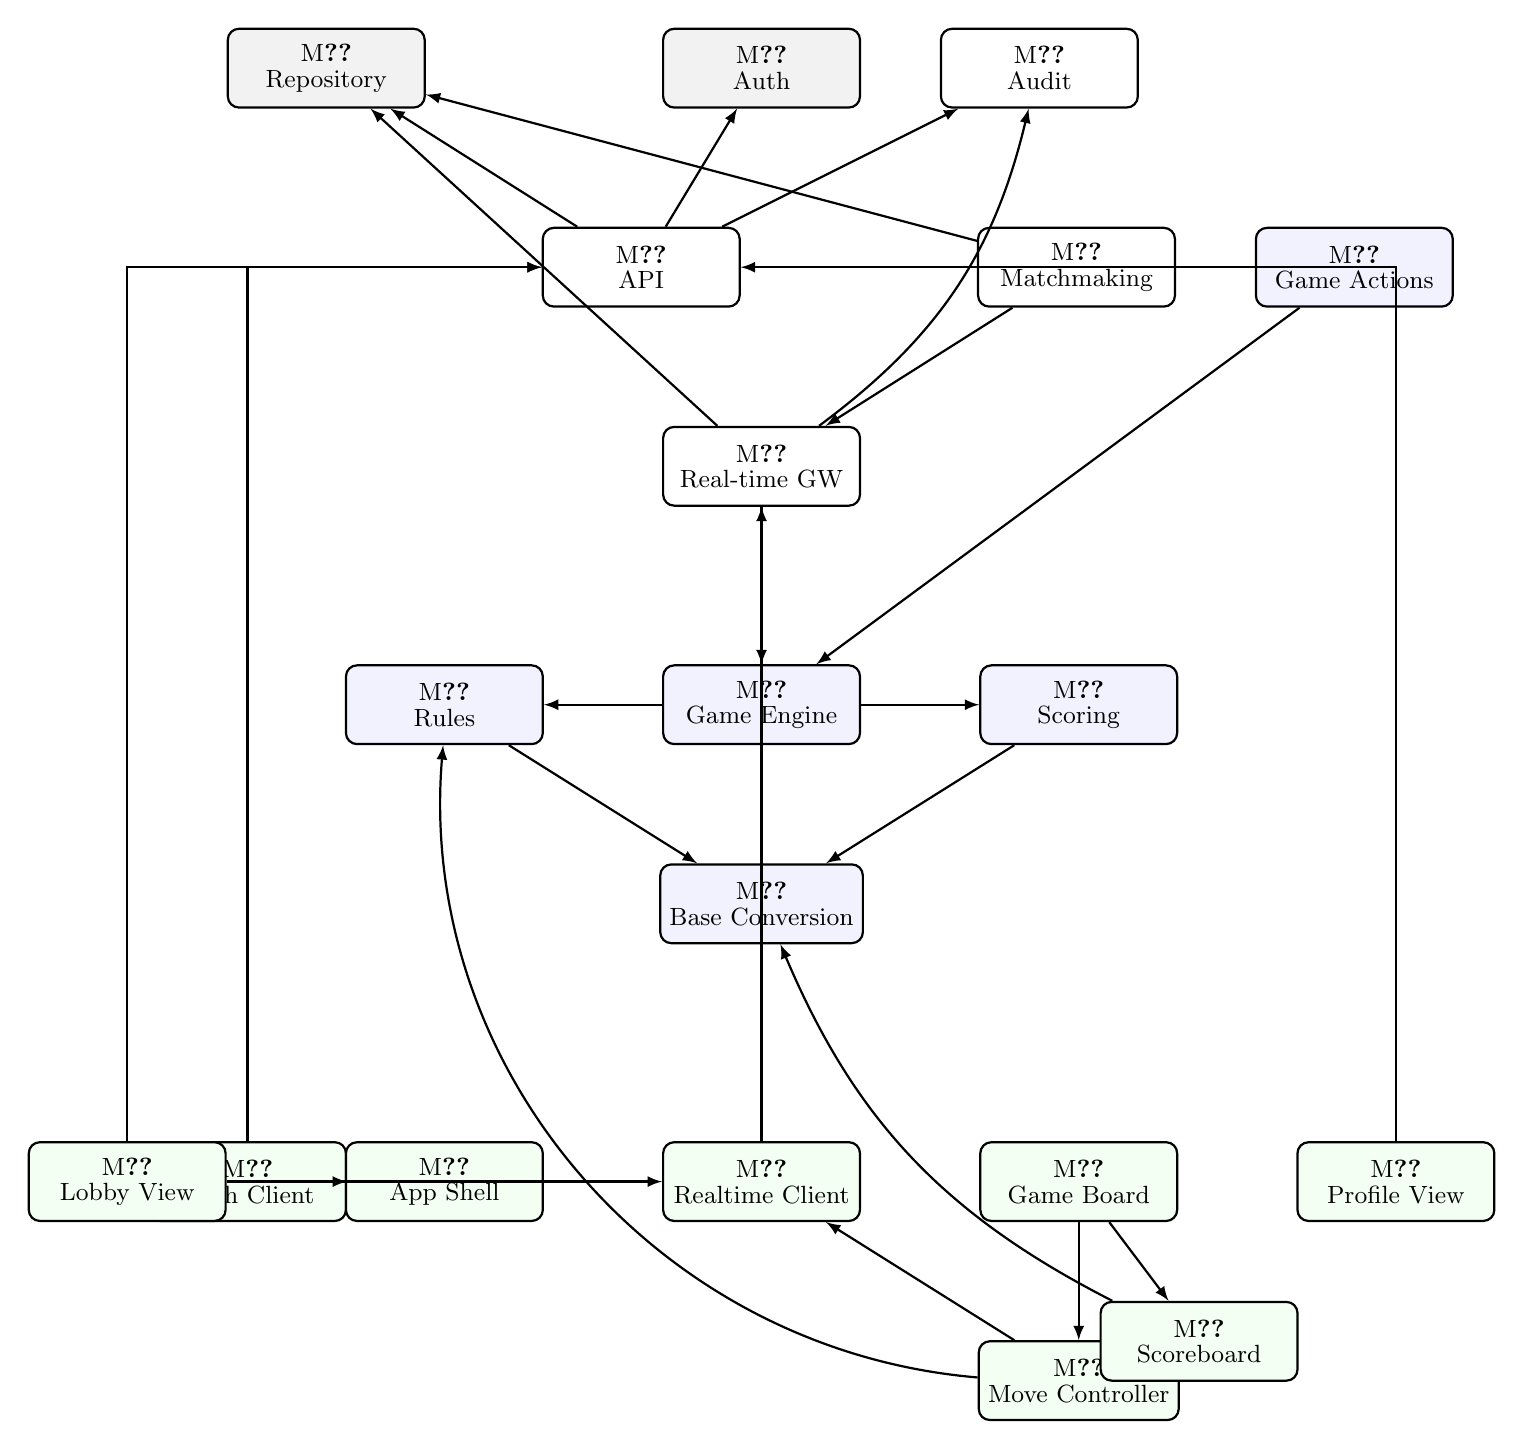
\begin{tikzpicture}[
    node distance=1.5cm and 1.5cm, % Vertical and Horizontal spacing
    auto, >=latex, thick,
    module/.style={
        rectangle, draw=black, rounded corners, fill=white,
        align=center, minimum height=1cm, minimum width=2.5cm,
        font=\small
    },
    % Group styles for visual distinction
    env/.style={module, fill=gray!10},   % Environment/Databases
    logic/.style={module, fill=blue!5},  % Core Logic
    ui/.style={module, fill=green!5}     % Frontend/UI
]

    % --- LEVEL 1: Persistence & External (Top) ---
    % Placing Repository centrally at top left-ish
    \node[env] (Repo) {\shortstack{\mref{mRepository}\\Repository}};
    \node[env] (Auth) [right=3cm of Repo] {\shortstack{\mref{mAuth}\\Auth}};
    \node[module] (Audit) [right=1cm of Auth] {\shortstack{\mref{mAudit}\\Audit}};

    % --- LEVEL 2: Server Entry Points ---
    % API uses Repo and Auth, so place it below them
    \node[module] (API) [below left=1.5cm and -1cm of Auth] {\shortstack{\mref{mAPI}\\API}};
    \node[module] (Matchmaking) [right=3cm of API] {\shortstack{\mref{mMatchmaking}\\Matchmaking}};
    
    % Realtime GW is central
    \node[module] (RealtimeGW) [below right=1.5cm and -1cm of API] {\shortstack{\mref{mRealtimeGateway}\\Real-time GW}};

    % --- LEVEL 3: Core Game Logic (Server) ---
    \node[logic] (GameEngine) [below=2cm of RealtimeGW] {\shortstack{\mref{mGameEngine}\\Game Engine}};
    \node[logic] (Rules) [left=1.5cm of GameEngine] {\shortstack{\mref{mRules}\\Rules}};
    \node[logic] (Scoring) [right=1.5cm of GameEngine] {\shortstack{\mref{mScoring}\\Scoring}};
    \node[logic] (GameActions) [right=1cm of Matchmaking] {\shortstack{\mref{mGameActions}\\Game Actions}};
    
    % Base Conversion is a utility used by Rules/Scoring, place below them
    \node[logic] (BaseConv) [below=1.5cm of GameEngine] {\shortstack{\mref{mBaseConversion}\\Base Conversion}};

    % --- LEVEL 4: Frontend Network Layer ---
    \node[ui] (RealtimeClient) [below=2.5cm of BaseConv] {\shortstack{\mref{mRealtimeClient}\\Realtime Client}};
    \node[ui] (AuthClient) [left=4cm of RealtimeClient] {\shortstack{\mref{mAuthClient}\\Auth Client}};

    % --- LEVEL 5: Frontend UI Views ---
    \node[ui] (AppShell) [left=1.5cm of RealtimeClient] {\shortstack{\mref{mAppShell}\\App Shell}};
    \node[ui] (LobbyView) [left=1.5cm of AppShell] {\shortstack{\mref{mLobbyView}\\Lobby View}};
    
    \node[ui] (GameBoard) [right=1.5cm of RealtimeClient] {\shortstack{\mref{mGameBoardView}\\Game Board}};
    \node[ui] (ProfileView) [right=1.5cm of GameBoard] {\shortstack{\mref{mProfileView}\\Profile View}};

    % --- LEVEL 6: Frontend Interactions ---
    \node[ui] (MoveCtrl) [below=1.5cm of GameBoard] {\shortstack{\mref{mMoveController}\\Move Controller}};
    \node[ui] (Scoreboard) [below right=1cm and -1cm of GameBoard] {\shortstack{\mref{mScoreboardView}\\Scoreboard}};


    % --- EDGES (Arrows) ---

    % Server Backend Edges
    \draw[->] (API) -- (Repo);
    \draw[->] (API) -- (Auth);
    \draw[->] (API) -- (Audit);
    
    \draw[->] (RealtimeGW) -- (Repo);
    \draw[->] (RealtimeGW) edge[bend right=20] (Audit);
    \draw[->] (RealtimeGW) -- (GameEngine);
    
    \draw[->] (Matchmaking) -- (Repo);
    \draw[->] (Matchmaking) -- (RealtimeGW);

    % Game Logic Edges
    \draw[->] (GameEngine) -- (Rules);
    \draw[->] (GameEngine) -- (Scoring);
    \draw[->] (Rules) -- (BaseConv);
    \draw[->] (Scoring) -- (BaseConv);
    \draw[->] (GameActions) -- (GameEngine);

    % Frontend -> Backend Cross-over
    % We use loose dashed lines or standard lines for network calls
    \draw[->] (AuthClient) |- (API);
    \draw[->] (RealtimeClient) -- (RealtimeGW);

    % Frontend Internal Edges
    \draw[->] (AppShell) -- (AuthClient);
    \draw[->] (LobbyView) -- (RealtimeClient);
    \draw[->] (LobbyView) |- (API); % Lobby uses API to list rooms
    
    \draw[->] (GameBoard) -- (MoveCtrl);
    \draw[->] (GameBoard) -- (Scoreboard);
    
    \draw[->] (MoveCtrl) -- (RealtimeClient);
    % MoveCtrl locally validates with rules (optional arrow if client-side validation exists)
    \draw[->] (MoveCtrl) edge[bend left=45] (Rules); 

    \draw[->] (Scoreboard) edge[bend left=20] (BaseConv);
    \draw[->] (ProfileView) |- (API);

\end{tikzpicture}
\caption{Use hierarchy (DAG) showing primary ``uses'' relations between modules.}
\label{FigUsesDAG}
\end{figure}

\bigskip
\noindent\textbf{Design rationale:} The DAG above shows the server-authoritative pattern: Realtime gateway owns live interactions and forwards validated moves to the Game Engine; the Game Engine uses the Rules and Scoring modules, and persistence is abstracted via the Repository. Frontend views rely on the Realtime client for live updates and the API for non-realtime operations (profile, auth, lobby listing).

\newpage
%\includegraphics[width=0.7\textwidth]{UsesHierarchy.png}



\newpage
\section{User Interfaces (UI) --- sketches and wireframes} \label{SecUI}

\begin{figure}[H]
\centering
\includegraphics[width=0.85\textwidth]{Crazy10s_basic_game_UI.png}
\caption{Hand-drawn / mockup: Game board layout (commented out until image is available).}
\label{FigUIimage}
\end{figure}


\section{Design of Communication Protocols} \label{SecCP}

This section captures the protocol-level design for server-client communication, with a focus on login/auth flows (REST) and gameplay flows (WebSocket). The approach favours a server-authoritative model: the server is the source of truth for game state.

\subsection{Authentication and Profile (REST)}
\paragraph{Endpoints (HTTP/JSON)}
\begin{itemize}
  \item \texttt{POST /api/auth/signup} \{ username, password \} $\rightarrow$ 201 / error
  \item \texttt{POST /api/auth/login} \{ username, password \} $\rightarrow$ \{ token, user \}
  \item \texttt{POST /api/auth/guest} $\rightarrow$ \{ token, guestId \}
  \item \texttt{GET /api/profile/:userId} Authorization: Bearer token $\rightarrow$ profile
  \item \texttt{PUT /api/profile/:userId} Authorization: Bearer token $\rightarrow$ updated profile
\end{itemize}

\noindent\textbf{Auth notes:} JWT-like Bearer tokens are issued on login and short-lived (configurable). Refresh tokens are out-of-scope for MVP but supported in design. Tokens are stored in secure HTTP-only cookies or in-memory (client decision in \mref{mAuthClient}).

\subsection{Real-time Gameplay (WebSocket / Socket.IO style)}
\paragraph{Connection lifecycle}
\begin{enumerate}
  \item Client connects to the Realtime Gateway with an Authorization header (Bearer token).
  \item Server validates token, optionally checks profile/permissions, and assigns the socket to the user's session.
  \item Client requests to join or create a lobby room via \texttt{joinRoom / createRoom}.
\end{enumerate}

\paragraph{Message schema (JSON) --- examples}
\begin{itemize}
  \item \textbf{Client $\rightarrow$ Server:} \texttt{\{ type: "playCard", payload: \{ sessionId, action: \{ kind:"play", card:\{suit,rank\}, meta:\{\}\} \} \}}
  \item \textbf{Client $\rightarrow$ Server:} \texttt{\{ type: "drawCard", payload: \{ sessionId \} \}}
  \item \textbf{Server $\rightarrow$ Client:} \texttt{\{ type: "stateUpdate", payload: \{ sessionId, state: \{ hands, discardTop, turn, scores\} \} \}}
%  \item \textbf{Server $\rightarrow$ Client:} \texttt{\{ type: "actionResult", payload: \{ ok: true/false, reason?: "invalid_move" \} \}}
%  \item \textbf{Server -> Client:} \texttt{\{ type: ``reconnectSnapshot'', payload: \{ sessionId, fullState \} \}} (used on reconnection)
\end{itemize}

\paragraph{Protocol properties and constraints}
\begin{itemize}
  \item \textbf{Authoritative server:} All move validation occurs on the server (\mref{mRules}/\mref{mGameEngine}). Clients may do local pre-checks for responsiveness, but final acceptance comes from the server.
  \item \textbf{Idempotency:} Actions include client-generated request IDs so duplicate deliveries during reconnection are ignored.
  \item \textbf{Delta updates:} For performance, \texttt{stateUpdate} messages typically contain deltas; full-state snapshots are reserved for joins/reconnects.
  \item \textbf{Resync strategy:} On reconnect, the client requests a \texttt{reconnectSnapshot}. The server supplies a full state and the client applies it atomically to avoid inconsistent UI states.
  \item \textbf{Security:} All WebSocket connections are over WSS (TLS). Authorization is checked per message where required.
\end{itemize}

\subsection{Sequence Example: Play Card flow}
\begin{enumerate}
  \item Client sends \texttt{playCard} with action payload.
  \item Realtime Gateway authenticates and forwards the action to Game Engine worker.
  \item Game Engine validates via Rules module:
    \begin{itemize}
      \item If accepted: update state, persist via Repository, emit \texttt{actionResult(ok:true)}, then emit \texttt{stateUpdate} to all room clients.
%      \item If rejected: emit \texttt{actionResult(ok:false, reason:"invalid_move")} to the initiating client.
    \end{itemize}
\end{enumerate}

\subsection{Failure modes and mitigation}
\begin{itemize}
  \item \textbf{Dropped messages / short disconnects:} idempotent request IDs plus reconnection snapshot mitigate lost messages.
  \item \textbf{Lag / delayed updates:} server sends small heartbeats and uses sequence numbers so clients can detect missing updates.
  \item \textbf{Untrusted clients:} server always re-checks any client-supplied action against the Rules module — never trust client state for authoritative decisions.
\end{itemize}

\section{Timeline}

%%add

\newpage

\bibliographystyle {plainnat}
\bibliography{../../../refs/References}

\end{document}